\documentclass[11pt]{article}
\usepackage{tikz}
\usepackage[height=220mm, width=165mm]{geometry}
%% \usetikzlibrary{calc}

\usepackage{graphicx}
\usepackage{fancyhdr}
\usepackage{xcolor}
\usepackage{listings}
\usepackage{multicol}

\usepackage{amsmath}
%% \usepackage{algorithm}
%% \usepackage[noend]{algpseudocode}

\setlength{\headheight}{15pt}

\pagestyle{fancy}
\lhead{Assignment 9}
\rhead{Kevin Mooney -- 11372946}
\fancyfoot{}

\linespread{1.3}

\lstset{language=C++,
                keywordstyle=\color{blue},
                morekeywords={REAL, __global__},
                stringstyle=\color{red},
                commentstyle=\color{green!50!black},
                morecomment=[l][\color{magenta}]{\#},
                frame=single
}




\begin{document}

\vspace*{3mm}
\noindent
{\centering\textbf{\Large N-body Simulation}\\}
\vspace*{8mm}

\section*{Compiling \& Running - \texttt{make}}
The source code can be found in src with a corresponding makefile so the program can be compiled by simply running \verb!make!. A sample execution of the program is as such 
\begin{itemize}
\item[\$] \texttt{mpirun -n 9 ./n-body -n 18 -s 1000 -w 10 -h 10}
\end{itemize}  
This sets the number of particles to 18, the number of iterations to 1000, the width to 10 and height to 10. An animation showing a problem with 96 particles and 8 processes can be found in the images directory. It's called animation.gif.

\subsection*{Outline of Problem}

The Lennard-Jones potential has the form
\begin{equation}
  V_{\textrm{LJ}}(r) = 4\epsilon\left[\left(\frac{\sigma}{r}\right)^{12} 
                  - \left(\frac{\sigma}{r} \right)^6\right]
\end{equation}
where epsilon is the depth of the potential well and sigma is the point at which the inter-particle potential is 0. As for our simulation we aren't concerned with making any measurements, the potential can be simplified to 

\begin{equation}
  V_{\textrm{LJ}}(r) = \frac{1}{12}\left[r^{-12} - 2{r}^{-6}\right]
\end{equation}
Which makes the force easy to calculate using

\begin{equation}
  \vec{F}(r) = \left[r^{-13} - {r}^{-7}\right] \hat{r}
\end{equation}
Using a leap frog routine with a sufficiently small time step conserves energy.
\pagebreak
\section*{Serial Simulation}

For the serial implementaion, each point had a structure associated with it that stored it's position, velocity and net force exerted on it. Periodic boundary conditions were used but particles were allowed to stray out of the box. Taking two particles, the closest distance between the particles could be calculated by taking the actual distance between the two particles and dividing this by the width of the box. This was then rounded to the nearest integer, telling us how many ``boxes'' outside the particle was, allowing the distance to be scaled accordingly. Each pair of particles was only looked at once each iteration. The code for the pairwise update is as follows

\small
\begin{lstlisting}
inline void update_pairwise_force 
  ( POINT *p1, POINT *p2, REAL (*f)(REAL), double width, double height ) {
  REAL fx, fy, dx, dy, total_force, radial_seperation;

  /* Find closest dx, shamelessly stolen from wikipedia */
  dx  = p2->rx - p1->rx;
  dy  = p2->ry - p1->ry;
  dx -= width  * round ( dx / width  ); /* could precalculate */
  dy -= height * round ( dy / height );

  radial_seperation = sqrt ( dx*dx + dy*dy );
  total_force       = - f ( radial_seperation );
  fx = total_force * ( dx ) / radial_seperation;
  fy = total_force * ( dy ) / radial_seperation;

  /* Append forces */
  p1->fx += fx;
  p1->fy += fy;
  p2->fx -= fx;
  p2->fy -= fy;
}
\end{lstlisting}
\normalsize
The particles were then confined to the box when printed to a file

\pagebreak

\section*{Parallel Implementation}

For the MPI part of the homework I set up a cartesian topology. All data for the MPI is initialised at the start and is stored in a mega struct found in para\_grid.h. Each process is given a certain region to be in charge of. Every particle in each process is aware of every particle in the process and any particles within a certain delta of it's processors region. Thus for the communication, first any particle that has changed region is sent over, then any particle near a neighbouring region has it's coordinates sent over. This specific procedure doesn't scale well on a single process but scales well as the number of processes increases as each process only has to consider a fraction of the particles. A graph of the strong scaling behaviour can be seen in figure 1, it shows that the problem scales well as the number of processes increases. The routine on the single process could be improved by also implementing the cut-off point in each process, which the parallel algorithm would benefit from too.

\begin{figure}[h]
  \centering
  \caption{Strong scaling of program for various point counts}
  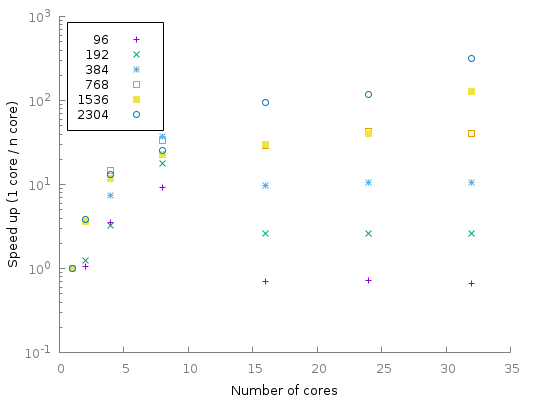
\includegraphics[width=0.7\textwidth]{../images/speedup.png}
\end{figure}

\pagebreak

\section*{Bugs and Possible Improvements}

\begin{itemize}
\item Currently the size of the halo buffers as well as some other arrays is hard coded. This is bad and means the problem won't work for larger sizes and different number of dimensions. 
\item The cut-off point is only implemented from region to region and not within a process. An efficient way of implementing the cut-off point would be to keep the points sorted. This would also make finding the halos easier.
\end{itemize}

\end{document}
